% HMC Math dept HW template example
% v0.04 by Eric J. Malm, 10 Mar 2005
\documentclass[12pt,letterpaper,boxed,cm]{hmcpset}

% set 1-inch margins in the document
\usepackage[margin=1in]{geometry}
\usepackage{mathtools}
\usepackage{mathrsfs}
% include this if you want to import graphics files with /includegraphics
\usepackage{graphicx}
\usepackage{cases}
\usepackage{hyperref}
\usepackage{siunitx}
\usepackage{tikz}
\usepackage{cases}
\usetikzlibrary{arrows}

% info for header block in upper right hand corner
\name{Name: ~~~~~~~~~~~~~~~~~~~~~}
\class{Physics 51}
\assignment{Homework \#10}
\duedate{October 6, 2016}

\newcommand{\ev}[2]{\Big|_{#1}^{#2}}
\newcommand{\evv}[2]{\Big|_{#1}^{#2}}
\newcommand{\set}[1]{\left\{#1\right\}}
\newcommand{\s}[1]{\sqrt{#1}}
\newcommand{\f}[2]{\frac{#1}{#2}}
\newcommand{\p}[2]{\frac{\partial #1}{\partial #2}}
\providecommand{\t}[1]{\text{#1}}
\providecommand{\span}[1]{\text{span}\left(#1\right)}
\providecommand{\set}[1]{\left\{#1\right\}}
\providecommand{\l}[0]{\left}
\providecommand{\r}[0]{\right}
\newcommand{\m}[1]{\begin{matrix}#1\end{matrix}}
\newcommand{\bm}[1]{\begin{bmatrix}#1\end{bmatrix}}
\renewcommand{\bf}[1]{\mathbf{#1}}
\newcommand{\pn}[1]{\left( #1 \right)}
\newcommand{\abs}[1]{\left| #1 \right|}
\newcommand{\bk}[1]{\left[ #1 \right]}
\newcommand{\cis}[1]{\pn{\cos\pn{#1} + i\sin\pn{#1}}}
\newcommand{\cisi}[1]{\pn{\cos\pn{#1} - i\sin\pn{#1}}}
\renewcommand{\Im}[1]{\text{Im}\pn{#1}}
\renewcommand{\Re}[1]{\text{Re}\pn{#1}}
\renewcommand{\k}[0]{\f{1}{4\pi\epsilon_0}}
\renewcommand{\part}[1]{\vspace{1em}\noindent(#1)}

\makeatletter
\renewcommand*\env@matrix[1][*\c@MaxMatrixCols c]{%
  \hskip -\arraycolsep
  \let\@ifnextchar\new@ifnextchar
  \array{#1}}
\makeatother
\begin{document}
\problemlist{33-E20, 33-P2}

\begin{problem}[33-E20]
	\begin{enumerate}
		\item[(a)] A long wire is bent into the shape shown in Fig. 33-46, without cross contact at $P$. The radius of the circular section is $R$. Determine the magnitude and direction of $\vec{\mathbf{B}}$ at the center $C$ of the circular portion when the current $i$ is as indicated.
		\item[(b)] The circular part of the wire is rotated without distortion about the dashed line one quarter turn clockwise as   viewed from above, so that the plane of the circular loop is now perpendicular to the plane of the page. Determine $\vec{\mathbf{B}}$ at $C$ in this case.
	\end{enumerate}	
	\begin{center}
		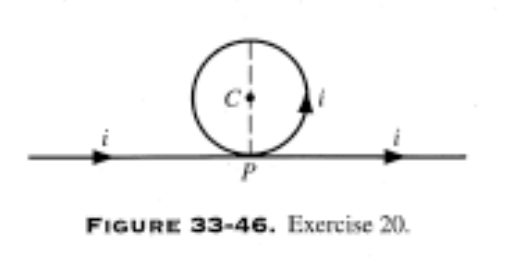
\includegraphics[scale=0.7]{01.png}
	\end{center}
\end{problem}
\begin{solution}
\end{solution}
\newpage

\begin{problem}[33-P2]
 A straight section of wire of length $L$ carries a current $i$. 
 \begin{enumerate}
 	\item[(a)] Show that the magnetic field associated with this segment at $P$, a perpendicular distance $D$ from one end of the wire (see Fig. 33-58), is given by
 	\[
 		B = \f{\mu_0 i}{4\pi D} \f{L}{\pn{L^2+D^2}^{1/2}}.
 	\]	
 	\item[(b)] Show that the magnetic field is zero at point $Q$, along the line of the wire.
 \end{enumerate}	
	\begin{center}
		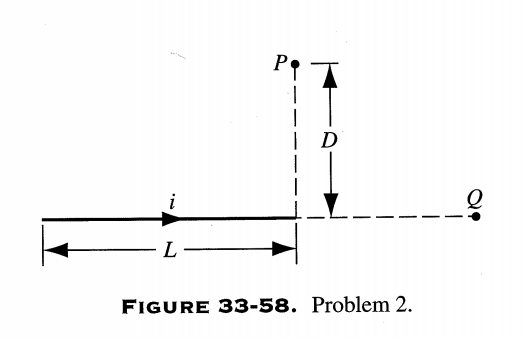
\includegraphics[scale=0.7]{02.png}
	\end{center}
\end{problem}
\begin{solution}
\end{solution}


\end{document}